\chapter{Assistentes de Provas}
	\label{cap:AssistentesProvas}
	Segundo~\citeshort{geuvers2009proof}, assistentes de provas\footnote{Também chamados de provadores semi-automáticos de teoremas ou provadores interativos.}
	são sistemas computacionais que permitem usuários definirem, provarem propriedades e
	raciocinarem sobre teorias e objetos matemáticos.~\citeshort{harrison2014history} descrevem como um sistema que um humano usa interativamente para produzir
	provas formais. Já~\citeshort{silva2019certificacao} descreve como programas que auxiliam no desenvolvimento de provas formais, mas não as fazem automaticamente e
	necessitam de um humano para guiar a prova.

	Segundo~\citeshort{harrison2014history} o conceito de assistentes de provas surge durante os anos de 1960 e 1970, a partir do reconhecimento que a capacidade de provadores
	automáticos de teoremas estavam estagnando, apesar de grande atividade e inovação na área. Provadores automáticos de teoremas, ao contrário de assistentes de provas,
	são softwares que automaticamente geram, se possível, provas para expressões matemáticas, geralmente por um método de busca em um domínio específico.
	De acordo com~\citeshort{harrison2014history} e~\citeshort{geuvers2009proof}, durante este período surgiram os primeiros assistentes de provas, dentre eles estão Automath, LCF, Mizar e PVS.

	De acordo com~\citeshort{silva2019certificacao}, provas assistidas por computador inicialmente não foram bem recebidas pela comunidade matemática, pois o objetivo de uma prova é
	convencer um leitor que algo é verdadeiro e explicar o porquê, algo que provas desenvolvidas em computador não são bem adaptadas, pois, em geral,
	suas linguagens internas não são de fácil entendimento. Porém, diversos resultados importantes foram provados em assistentes de provas, segundo~\citeshort{geuvers2009proof},
	o teorema da Curva de Jordan foi provado em ambos Mizar e HOL Light, o Teorema dos Números Primos foi provado em Isabelle e o Teorema das Quatro Cores foi provado em Coq.

	É de interesse analisar mais este último teorema, pois foi o primeiro grande resultado provado em um computador. Em específico, o problema foi detalhado e alguns casos foram provados
	em~\citeshort{appel1976every} e outros casos, além de uma prova em computador (em linguagem \textit{assembly} para computadores IBM 370), foi apresentada em~\citeshort{appel1977every}.
	O motivo da prova ter sido realizada em um computador é devido à quantidade de casos a serem analisados, cerca de 1 bilhão de acordo com~\citeshort{gonthier2005computer}.

	A prova de~\citeauthoronline{appel1977every} não foi imediatamente aceita pela comunidade matemática, apenas com a publicação de uma monografia definitiva da prova
	em~\citeshort{appel1989every} e com a prova de~\citeshort{robertson1997four}, também em computador mas muito mais simples e feita na linguagem C, o Teorema
	das Quatro Cores foi considerado provado~\cite{gonthier2005computer}. Por fim,~\citeshort{gonthier2005computer} formalizou a prova de~\citeauthoronline{robertson1997four} em Coq, dando,
	o que o autor descreve, como o passo final na prova. Ao longo dos anos, provas formalizadas em computador conseguiram reconhecimento, pois se
	demonstraram mais confiáveis que provas tradicionais.

	Assistentes de provas também são amplamente usados para verificar componentes de software, segundo~\citeshort{avigad2017theorem} \textit{verificação formal}
	consiste no uso de métodos matemáticos e computacionais para expressar afirmações em termos matemáticos precisos. Essas afirmações podem se referir à corretude
	de certos sistemas de software ou hardware ou à garantia de que um certo estado de um programa nunca será atingido, estes que, ao serem expressos em termos matemáticos,
	podem ser demonstrados por meio de assistentes de provas.

	Segundo~\citeshort{silva2019certificacao}, assistentes de provas tem propriedades interessantes, por exemplo, verificação rápida e mecânica de provas,
	comandos de busca de teoremas e lemas e automatização de provas. Uma propriedade que alguns assistentes de provas compartilham
	(por exemplo Coq~\cite{coqteam2022manual} e Lean~\cite{avigad2017theorem,demoura2015lean}) é satisfazer critério de de Bruijn. O critério afirma que o programa
	verificador de um assistente (seu \textit{kernel} ou \textit{núcleo}) deve ser um programa muito pequeno, que pode ser verificado manualmente, seja por meio de papel e caneta ou por
	um algoritmo simples que uma pessoa cética poderia desenvolver facilmente~\cite{barendregt2001proof}. O verificador deve gerar algum tipo de ``objeto de prova'',
	por exemplo um termo \(\lambda\), que pode ter sua veracidade comprovada da mesma forma que o verificador de tipos.

	Neste capítulo, será apresentado o conceito de teoria de tipos e o assistente de provas Coq será descrito. Na Seção~\ref{sec:TeoriaTipos} será
	brevemente apresentada a Teoria de Tipos e na Seção~\ref{sec:Coq} será descrito o assistente de provas Coq.

	\section{Uma Breve Apresentação de Teoria de Tipos}
		\label{sec:TeoriaTipos}
		Teoria dos tipos surge, de acordo com~\citeshort{sep-type-theory}, como uma tentativa de Russell para lidar com o Paradoxo de Russell:
		sendo \(R = \{ x \ | \ x \notin x\}\) então \( R \in R \tofrom R \notin R\), presente na Teoria de Conjuntos.
		O cerne do paradoxo se encontra na quantificação de \textit{x} na definição de \textit{R}, em específico, \textit{x} é quantificado sobre
		todos os conjuntos, o que inclui o próprio conjunto \textit{R}, possibilitando então que \textit{x} seja instanciado como \textit{R}.

		Em uma carta para Frege escrita em 1902, Russell comunica a descoberta do paradoxo e indica que o problema está relacionado com a quantificação
		de objetos; Frege responde à Russell menos de uma semana depois, indicando que uma possível solução para o problema lidaria com ``níveis'' de objetos,
		assim impedindo que um objeto de um dado nível possa quantificar sobre objetos de níveis diferentes~\cite{van2002frege}. Porém, uma proposta de solução ao paradoxo
		surge apenas no apêndice B de~\citeshort{russell1903principles}\footnote{É de interesse ressaltar a seguinte passagem do livro, presente no Apêndice A,
		página 762: ``\textit{A variable will not be able, except in special cases, to extend from one of these sets into another; and in \(x \in u\), the
		x and the u must always belong to different types}[...]''.} onde Russell introduz provisoriamente a ``Doutrina de Tipos'',
		o que eventualmente se tornou a Teoria de Tipos moderna.

		Após explorar diversas outras teorias para lidar com os paradoxos da Teoria de Conjuntos~\cite{van2002frege}, Russell voltou a trabalhar
		na teoria de tipos, resultando na Teoria de Tipos Ramificada~\cite{russell1908mathematical}. Porém, problemas presentes nesta
		teoria\footnote{Para mais detalhes sobre, veja~\cite[p. 150-153]{van2002frege}.} levaram \citeshort{ramsey1931general} a desenvolver
		a Teoria de Tipos Simples, que é uma versão mais restrita da Teoria de Tipos Ramificada.

		A Teoria de Tipos Simples foi reformulada por Church~\cite{church1940formulation} para desenvolver a sua própria versão da teoria de
		tipos, usando a sintaxe do \CalcLambda, o que hoje é chamado de \CLST~\cite{huet1990logical}. Na sua formulação, novos tipos
		são definidos indutivamente a partir de dois tipos básicos, (\textit{i} para indivíduos e \textit{o} para proposições) e de uma regra
		de definição de tipos (sendo \textit{A} e \textit{B} tipos, então toda função \(A \to B\) de \textit{A} para \textit{B} é um tipo).
		Predicados tem tipo \(i \to o\) e funções tem tipo \(i \to i\). Por fim, expressões são definidas a partir de uma linguagem de \CalcLambda estendida para
		lidar com tipos.

		Segundo~\citeshort{howard1980formulae},~\citeshort{curry1958combinatory} apontaram uma correspondência direta entre axiomas do fragmento positivo implicativo
		de lógica proposicional e combinadores do \CalcLambda, já~\citeshort{tait1967intensional} observou uma correspondência direta entre a regra de eliminação do corte
		em Cálculo de Sequentes e redução de Termos \(\lambda\). \citeshort{howard1980formulae} então demonstrou, com base nestes resultados, que há uma
		correspondência direta entre a Lógica Intuicionista (descrita sintaticamente como um cálculo de sequentes) e o \CalcLambda Simplesmente Tipado,
		dando surgimento ao que hoje é chamado de Correspondência de Curry-Howard\footnote{Essa noção é expandida por Wadler~\cite{wadler2015propositions}
		onde o autor defende que a Correspondência é apenas um nome para um fenômeno maior chamado de \textit{Propositions as Types}
		(Proposições como Tipos).}.

		Na década de 1970 foi desenvolvido um novo tipo de \CalcLambda tipado, chamado de Sistema F ou \CalcLambda de Segunda Ordem, independentemente por~\citeshort{girard1971extension}
		e~\citeshort{reynolds1974towards}. Este sistema estende o \CLST adicionando uma operação de abstração de tipos, permitindo definir termos \(\lambda\)
		com variáveis que podem ser instanciadas como um tipo~\cite{girard1989proofs}. Isso se mostrou especialmente útil para a computação, em específico
		para a formalização do conceito de funções polimórficas.

		Pouco tempo após o desenvolvimento do Sistema F,~\citeauthoronline{girard1972interpretation} apresentou o Sistema \(\mathrm{F}_\omega\)~\cite{girard1972interpretation}
		que é uma generalização do Sistema F, adicionando os conceitos de construtores de tipos e \textit{kinds}\footnote{Pode ser traduzido como ``gênero''.}.
		Construtores de tipos são tipos especiais de funções que recebem tipos e retornam tipos, já \textit{kinds} podem ser entendidos como ``tipos de tipos'',
		essencialmente é uma cópia do \CLST a nível de tipos~\cite{pierce2002types}. As abstrações de tipos do Sistema F pode ser entendida
		como uma dependência de termos em tipos, já os construtores de tipos do Sistema \(\mathrm{F}_\omega\) pode ser entendidos como uma dependência
		entre tipos.

		Outro importante desenvolvimento na teoria de tipos foi a Teoria de Tipos Intuicionista ou Teoria de Tipos de Martin-Löf~\cite{martin1975intuitionistic,martin1984intuitionistic},
		proposta por~\citeauthoronline{martin1975intuitionistic} como um sistema lógico fundacional para a matemática construtivista, de forma análoga à
		Teoria de Conjuntos de Zermelo-Frankel para a matemática clássica. Uma das características deste sistema é uma distinção rigorosa entre proposições
		e julgamentos; proposições são objetos que podem ser combinados por meio de operações lógicas como \(\neg, \land, \lor, \to, \exists, \forall\), já
		julgamentos são afirmações sobre proposições. Por exemplo, na frase ``\PHI é verdadeiro'', \PHI é uma proposição e ``\PHI é verdadeiro'' é um
		julgamento~\cite{martin1984intuitionistic}.

		A \TTML está intimamente relacionada à \CCH, pois toda proposição em \TTML representa um tipo, o tipo de todas as provas da proposição. Por exemplo,
		a frase ``971 é um número não primo'' descreve a proposição que é provada fornecendo dois números naturais maiores que 1 e uma computação que mostra
		que seu produto é 971. Por outro lado, todo tipo também descreve uma proposição, em específico, a proposição que o tipo em questão não é vazio, que
		é provada fornecendo um objeto que habita o tipo~\cite{martin1975intuitionistic}. Ao provar uma proposição em \TTML, construímos um objeto que habita o tipo
		desta proposição, estes objetos são chamados de \textit{objetos de prova} e são ditos serem \textit{testemunhas} para a verdade da proposição~\cite{sep-type-theory-intuitionistic}.

		Duas noções importantes para a Teoria de Tipos são introduzidas na \TTML, são elas o Universo de Tipos e Tipos Dependentes. Universo de tipos é uma forma de lidar
		com a necessidade de criar tipos arbitrários dentro da linguagem. Existem duas famílias de tipos: os tipos pequenos e os tipos grandes, estas respeitam
		a seguinte hierarquia bem fundada: \(V_0 \in V_1 \in V_2 \in \dots \in V_n \in \dots\)\footnote{Aqui considere que a notação \(a \in B\) indica que \textit{B}
		é o tipo do objeto \textit{a}.}, sendo \(V_0\) a família dos tipos pequenos e toda família \(V_i, i \geq 1\) dos tipos grandes
		de ordem \textit{i}, onde todo \(V_n\) tem tipo \(V_{n+1}\)~\cite{martin1975intuitionistic}. É importante ressaltar que não é possível impor a restrição
		que um tipo seja um objeto dele mesmo, ou seja que \textit{V} tenha tipo \textit{V}, pois isso levaria a uma contradição semelhante ao Paradoxo de Russell~\cite{girard1972interpretation}.
		Uma variável de tipo em uma expressão é dita dependente se o tipo a qual ela será instanciada depende do valor de algum termo na expressão, nesse
		caso o tipo de toda a expressão é dito dependente~\cite{martin1975intuitionistic}.
		% Por exemplo, um predicado \(\mathrm{Primo}(x)\) que representa se o número
		% \textit{x} é ou não primo, depende do valor de \textit{x}, pois, caso \textit{x} seja um número primo, \(\mathrm{Primo}(x)\) será o tipo de provas
		% de que \textit{x} é primo, caso \textit{x} não seja primo, \(\mathrm{Primo}(x)\) será o tipo vazio.

		Segundo~\citeshort{coqteam2022manual},~\citeauthoronline{coquand1985constructions} uniram o sistema \(\mathrm{F}_\omega\) e a \TTML para criar o Cálculo de Construções (CoC),
		que é um sistema lógico baseado em teoria de tipos intuicionista com abstrações de tipos, construtores de tipos e tipos dependentes capaz de
		descrever indiretamente definições indutivas. Mais ainda, segundo~\citeshort{paulinmohring2015introduction}, o Cálculo de Construções é um sistema de tipos
		puro, ou seja, é um tipo de \CalcLambda com uma única linguagem que descreve ambos tipos e termos.

		Na Figura~\ref{fig:CuboLambda}, é apresentado um diagrama proposto originalmente por~\citeshort{barendregt1991introduction} para demonstrar relações entre
		diversos sistemas de tipos modernos. Cada flecha indica uma relação de inclusão (\(\subseteq\)) entre seus vértices, ou seja, o vértice de origem de uma flecha está incluso
		no vértice de destino da mesma. Uma das principais ideias no diagrama é representar as possíveis dependências mútuas entre tipos e termos, da seguinte forma:

		\begin{itemize}
			\item Tipos dependerem de termos (\(\rightarrow\))
			\item Termos dependerem de tipos (\(\uparrow\))
			\item Tipos dependerem de tipos (\(\nearrow\))
		\end{itemize}

		Como termos dependerem de outros termos é um componente básico do \CalcLambda, isso não é representado. Os sistemas de tipos representados são os seguintes:

		\begin{itemize}
			\item \(\lambda{\to}\): \CLST;
			\item \(\lambda 2\): Sistema F;
			\item \(\lambda\omega\): Sistema \(\mathrm{F}_{\omega}\);
			\begin{itemize}
				\item \(\lambda\underline{\omega}\): Uma versão mais fraca do Sistema \(\mathrm{F}_{\omega}\);
			\end{itemize}
			\item \(\lambda\Pi\): \textit{Logical Framework}, um sistema de \CalcLambda com tipos dependentes~\cite{harper1993framework};
			\item \(\lambda\mathrm{C}\): Cálculo de Construções.
		\end{itemize}

		\begin{figure}
			\centering
			\begin{tikzpicture}
				\matrix (m) [matrix of math nodes, row sep=3em, column sep=3em,
				text height=1.5ex,text depth=0.25ex]
				{
							& \lambda\omega             &              & \lambda\mathrm{C}            \\
				\lambda 2   &                           & \lambda\Pi 2                                \\
							& \lambda\underline{\omega} &              & \lambda\Pi\underline{\omega} \\
				\lambda{\to}&                           & \lambda\Pi  \\
				};
				\path[-{Latex[length=2.5mm, width=1.5mm]}]
				(m-1-2) edge (m-1-4)
				(m-2-1) edge (m-2-3)
						edge (m-1-2)
				(m-3-2) edge (m-1-2)
						edge (m-3-4)
				(m-4-1) edge (m-2-1)
						edge (m-3-2)
						edge (m-4-3)
				(m-3-4) edge (m-1-4)
				(m-2-3) edge (m-1-4)
				(m-4-3) edge (m-3-4)
						edge (m-2-3);
			\end{tikzpicture}
			\caption[Cubo \(\lambda\)]{Cubo \(\lambda\)\protect\footnotemark}
			\small{Fonte: Adaptado de~\cite{barendregt1991introduction}.}
			\label{fig:CuboLambda}
		\end{figure}
		\footnotetext{Diagrama originalmente produzido por Artem Pelenitsyn, de título original ``Lambda Cube'', gratuitamente disponível
		em \url{https://www.overleaf.com/latex/examples/lambda-cube/drnrtqnnjfzf}, licenciado pela licença Creative Commons CC BY 4.0 \url{https://creativecommons.org/licenses/by/4.0/deed.pt_BR}.}

		O Cálculo de Construções foi estendido por~\citeshort{coquand1988inductively} com a inclusão de definições indutivas primitivas, o que gerou o
		Cálculo de Construções Indutivas (CCI)~\cite{coqteam2022manual}. Este sistema de tipos é o formalismo por trás do Coq, todo objeto
		definido dentro do Coq é traduzido para um termo do CCI.

		Como apresentado em~\citeshort{coqteam2022manual}, no CCI, todo objeto tem um tipo, incluindo os próprios tipos.
		O tipo dos tipos se chama \textit{sort}\footnote{Pode ser traduzido adequadamente como ``classe''.}, e há uma hierarquia infinita e bem-fundada de \textit{sorts},
		onde os \textit{sorts} base são \textit{Set} e \textit{Prop}. Usaremos a notação \(A:\ B\) para denotar que o objeto \textit{A} tem tipo \textit{B}.

		O \textit{sort Set} é o tipo de todos os tipos pequenos, isto inclui tipos como o
		tipo dos números naturais e o tipo de termos booleanos, e também produtos, subconjuntos e funções sobre estes tipos. O \textit{sort Set} é o menor dos tipos.

		O \textit{sort Prop} é o tipo de proposições lógicas, onde um objeto \(\mathbb{P}: \textit{Prop}\) descreve uma classe de termos que representam
		provas de \Mathbb{P}, já um objeto \(\textit{p}: \mathbb{P}\) é dito uma \textit{testemunha} para a provabilidade da proposição \Mathbb{P}.
		Objetos em \textit{Prop} que não tem testemunhas são contradições.
		O \textit{sort SProp} é uma extensão do Coq originalmente proposta por \citeshort{gilbert2019definitional} que define uma classe de
		proposições estritas, estas são proposições cujas provas são irrelevantes (todas as provas são iguais).
		Ambos os \textit{sorts Prop} e \textit{SProp} são impredicativos, isto é, uma função que quantifica sobre todos os \textit{Props}/\textit{SProps} é
		também do tipo \textit{Prop}/\textit{SProp}. Formalmente, segundo~\citeshort{crosilla2017predicativity}, uma definição é impredicativa se define
		uma entidade por referência a alguma totalidade à qual a própria entidade pertence, e é predicativa caso contrário.

		Como \textit{Set} ser do tipo \textit{Set} gera uma teoria inconsistente, a linguagem do Cálculo de Construções Indutivas tem infinitos \textit{sorts}
		\(\textit{Type(i)}, i \geq 1\). Em particular, os \textit{sorts} \textit{Set}, \textit{Prop} e \textit{SProp} são do tipo \textit{Type(1)} e
		\(\forall i, \textit{Type(i)}: \textit{Type(i+1)}\). Os tipos são cumulativos, ou seja, para qualquer x, se \(x: \textit{Type(i)}\) então \(x: \textit{Type(i+1)}\),
		de forma análoga ao que ocorre na \TTML.

		% Uma característica importante do CCI são os tipos dependentes, que, segundo~\cite{pierce2002types}, podem ser entendidos como famílias de tipos que são
		% indexadas por termos, ou seja, o tipo de alguma expressão pode ser definido a partir do valor de algum termo.

	\section{O Assistente Coq}
		\label{sec:Coq}
		Coq é um assistente de provas para lógica de ordem superior desenvolvido desde 1984 por membros do instituto francês INRIA e seu \textit{kernel}
		é baseado no CCI. De acordo com~\citeshort{silva2019certificacao}, a Correspondência de Curry-Howard é o que
		dá versatilidade suficiente para o Coq para expressar lógicas mais sofisticadas, o autor ainda afirma que parte considerável
		da matemática pode ser expressa em Coq.

		Segundo~\citeshort{silva2019certificacao}, dentro da Ciência da Computação, Coq é usado principalmente como uma ferramenta para verificação de programas,
		como é o caso de~\citeshort{leroy2021compcert}, que desenvolveu um compilador para a linguagem C totalmente verificado em Coq, chamado de CompCert.
		Coq também pode ser usado para formalizar sistemas lógicos, como é o caso de~\citeshort{silveira2022sound} e~\citeshort{dewind2001modal} que descrevem a lógica modal alética
		em Coq e ~\citeshort{paiva1998temporal} que descreve a lógica temporal em Coq.

		De acordo com~\citeshort{silva2019certificacao}, Coq é tanto uma linguagem de programação funcional quanto uma linguagem de provas. Mais especificamente,
		Coq é composto dos seguintes componentes:
		\begin{itemize}
			\item \textit{Gallina}, que é uma linguagem de especificação e programação funcional, onde todo programa termina;
			\item \textit{Vernacular}, que é uma linguagem de comandos, permite interagir com o \textit{kernel} do Coq;
			\item Um conjunto de táticas para realizar provas, que são traduzidas para termos em \textit{Gallina};
			\item \Ltac, que é uma linguagem para implementação de táticas.
		\end{itemize}

		% Exemplos de provas / códigos
		Para utilizar o Coq de forma interativa, ferramentas como o CoqIDE\footnote{\url{https://coq.inria.fr/refman/practical-tools/coqide.html}.},
		VSCoq\footnote{\url{https://github.com/coq-community/vscoq}.} ou o ProofGeneral\footnote{\url{https://proofgeneral.github.io/}.} podem ser utilizadas.
		No que segue, serão apresentados exemplos feitos no CoqIDE, porém o mesmo se aplica às outras ferramentas.

		Para realizar uma prova em Coq usa-se os comandos \texttt{Theorem, Lemma, Example} ou \texttt{Corollary}\footnote{Internamente ao Coq todos são sinônimos, a
		distinção é apenas para os leitores.} para declarar uma expressão que será provada. Provas são iniciadas com o comando \texttt{Proof} e
		finalizadas com o comando \texttt{Qed} ou o comando \texttt{Defined}, mais ainda, provas podem ser aceitas sem serem completas com o comando
		\texttt{Admitted} e interrompidas com o comando \texttt{Abort}.

		Coq permite a definição indutiva de novos tipos, assim como a definição de funções recursivas e não recursivas. Tipos indutivos, definidos pelo comando
		\texttt{Inductive}, são definidos analogamente como na matemática ``tradicional'', onde é definido um conjunto de casos base para a indução e
		regras para a criação de novos objetos do tipo, onde ambos casos base e regras são chamados de construtores do tipo.
		Funções recursivas podem ser definidas pelo comando \texttt{Fixpoint}, estas operam sobre objetos de tipos indutivos podendo
		ter comportamentos diferentes dependendo de qual construtor de tipo foi usado para definir o objeto. Por fim, Coq também permite
		a definição de objetos arbitrários, com o comando \texttt{Definition}, que não passam da atribuição de um nome a algum termo~\cite{pierce2021software}.

		No desenvolvimento de provas interativas com o Coq uma prova pode ser verificada ``passo a passo'' pelo (\textit{kernel} do) Coq enquanto é desenvolvida (isto é, antes de
		ser finalizada). As ferramentas apresentadas anteriormente dispõem de duas janelas, uma janela de edição de texto,
		onde a prova de fato é escrita e uma janela de visualização, onde o estado da prova pode ser acompanhado, como pode ser visto com o caso do CoqIDE
		na Figura~\ref{fig:CoqIDEIntros}. O estado de uma prova é o conjunto de todas as hipóteses desta prova, assim como o conjunto de todos os termos que
		devem ser provados, chamados de \textit{goals} ou objetivos~\cite{coqteam2022manual}. O \textit{goal} pode ser separado em diversos \textit{subgoals}
		com a aplicação de algumas táticas, onde cada \textit{subgoal} deve ser provado para terminar a prova.
		A janela de visualização é dividida em duas partes por uma linha de inferência. Acima da linha estão as hipóteses e abaixo da linha está o \textit{goal},
		como pode ser visto na Figura~\ref{fig:CoqIDEIntros}.
		\begin{figure}[htpb!]
			\centering
			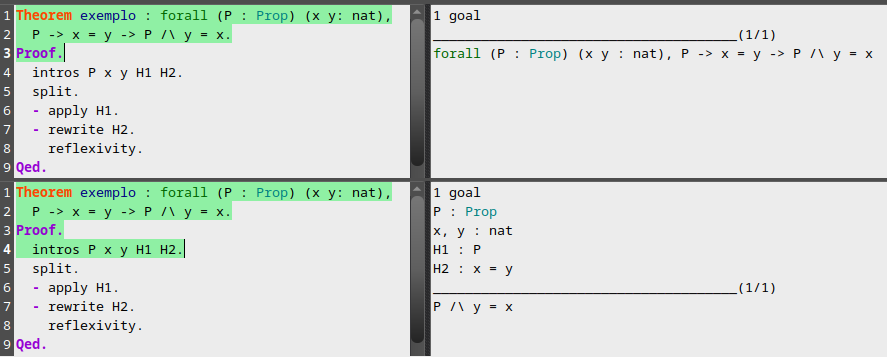
\includegraphics[scale=.5]{Figuras/CoqIDEIntrosJoin.png}
			\caption{Antes e depois de aplicar a tática \texttt{intros}.}
			\small{Fonte: \me}
			\label{fig:CoqIDEIntros}
		\end{figure}

		Durante o desenvolvimento interativo de provas, linhas são destacadas pela ferramenta que está sendo utilizada, a partir da resposta dada pelo verificador de tipos
		sobre o conteúdo daquela linha. Linhas destacadas em verde não geraram qualquer erro e foram aceitas pelo verificador de tipos, linhas destacadas em amarelo
		geraram algum tipo de aviso e linhas em vermelho foram rejeitadas pelo verificador de tipos, isto é, estão erradas de alguma forma.

		Na Figura~\ref{fig:CoqIDECores}, as linhas 13 e 15 até 17 estão destacas em amarelo pois não foram verificadas pelo verificador de tipos do Coq, isso é devido aos
		comandos \texttt{Admitted} e \texttt{Axiom}, que fazem com que os termos não sejam verificados pelo Coq e sejam tratados como verdades. A linha 23
		está destacada em vermelho pois ocorreu um erro nela, em específico, o Coq rejeitou a aplicação da tática \texttt{easy}. As restantes estão destacadas em verde
		pois foram aceitas pelo verificador de tipos.
		\begin{figure}[htpb!]
			\centering
			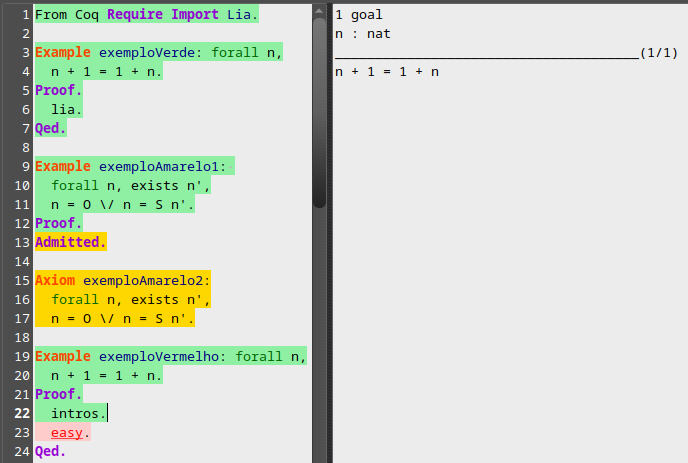
\includegraphics[scale=.5]{Figuras/CoqIDECores.png}
			\caption{Provas no CoqIDE.}
			\small{Fonte: \me}
			\label{fig:CoqIDECores}
		\end{figure}

		Dentro de provas no Coq, objetos são manipulados com táticas, por exemplo, a tática \texttt{intros} introduz termos quantificados universalmente
		no \textit{goal} e termos à esquerda de implicações\footnote{Estes na realidade são um caso particular de quantificação universal onde não há
		dependência de tipos entre o termo quantificado e a proposição sobre a qual ele está quantificado~\cite{pierce2021software}.} para o conjunto de hipóteses,
		a tática \texttt{apply} modifica o \textit{goal} ou as hipóteses com base no que está sendo aplicado e onde\footnote{Em específico, caso aplique-se um termo de tipo
		\(\texttt{A} \to \texttt{B}\) numa hipótese de tipo \texttt{A}, seus tipos serão unificados e a hipótese resultante terá tipo \texttt{B}, ou seja, equivale a aplicar
		a regra de modus ponens; caso aplique-se um termo de tipo \(\texttt{A} \to \texttt{B}\) num \textit{goal} de tipo \texttt{B}, seus tipos serão unificados e o
		\textit{goal} resultante terá tipo \texttt{A}, ou seja, é um tipo de \textit{backwards reasoning} - para provar \texttt{B} basta provar \texttt{A}.}
		e a tática \texttt{rewrite} reescreve equivalências no \textit{goal} ou em hipóteses.

		No que segue, conceitos de Coq serão apresentados por meio de exemplos práticos feitos pelo autor ou retirados de~\citeshort{pierce2021software}.

		\begin{exemplo}[Definições e Funções em Coq]
			Abaixo é definido indutivamente o tipo ``nat'' que representa os número naturais. Um número natural ou é \texttt{O} (representa o número 0) ou é o
			sucessor de outro número natural, representado como a aplicação da função sucessor \texttt{S} a algum número.
			A função recursiva ``plus'' apresenta a definição recursiva da soma de dois números naturais, já a função ``pred'' descreve uma operação de predecessor de um número.
			\begin{lstlisting}[language=coq]
		Inductive nat : Set :=
		  | O
		  | S: nat -> nat.
		Fixpoint plus (n : nat) (m : nat) : nat :=
		  match n with
		  | O => m
		  | S n' => S (plus n' m)
		  end.
		Definition pred (n : nat) : nat :=
		  match n with
		  | O => O
		  | S n' => n'
		  end.
			\end{lstlisting}
			Definições indutivas também podem ser utilizadas para descrever relações, como é o caso da relação ``ev'', representando paridade de números, abaixo.
			Esta definição descreve uma relação que associa números naturais (\texttt{nat}) à provas (\texttt{Prop}).
			\begin{lstlisting}[language=coq]
		Inductive ev : nat -> Prop :=
		  | ev_0 : ev 0
		  | ev_SS (n : nat) (H : ev n) : ev (S (S n)).
			\end{lstlisting}

			O construtor \texttt{ev\_SS} de \texttt{ev} requer \textit{evidências} para ser aplicado, em específico, ele requer um número natural \texttt{n} e uma prova
			\texttt{H} de \texttt{ev n}, ou seja, uma prova que \texttt{n} é par. Ao aplicar \texttt{ev\_SS} em algum termo, será necessário fornecer estas evidências
			para que verificador de tipos do Coq aceite a aplicação. \qed
		\end{exemplo}

		Para realizar provas em Coq, uma proposição é declarada, um nome é atribuído à ela e então um termo é construído a partir de axiomas,
		premissas e outros resultados já provados. Táticas são usadas para manipular estes e outros objetos relevantes para a prova até que esta seja concluída.
		Quando concluída, o termo provado é incluído no universo de fatos do Coq e pode ser utilizada em provas futuras.

		\begin{exemplo}[Provas em Coq]
			O teorema ``exemplo1'' mostra uma prova da comutatividade da disjunção lógica, já o lema ``exemplo2'' mostra uma prova indutiva que a soma de
			qualquer número natural com 0 é igual ao próprio número. Provas sobre relações indutivas podem ser feitas
			aplicando os construtores destas relações, no caso de \texttt{ev} do exemplo anterior, aplicando as regras \texttt{ev\_0} e \texttt{ev\_SS},
			como apresentado no corolário ``exemplo3'' abaixo, que prova que 4 é um número par.
			\begin{lstlisting}[language=coq]
		Theorem exemplo1: forall A B: Prop,
		  A \/ B -> B \/ A.
		Proof.
		  intros A B [HA | HB].
		  - right. assumption.
		  - left. assumption.
		Qed.
		Lemma exemplo2: forall n: nat,
		  n + 0 = n.
		Proof.
		  intros n.
		  induction n as [ | n' IHn].
		  - reflexivity.
		  - simpl. rewrite IHn. reflexivity.
		Qed.
		Corollary exemplo3: ev 4.
		Proof. apply ev_SS. apply ev_SS. apply ev_0. Qed.
			\end{lstlisting}
			\qed
		\end{exemplo}

		\subsection{Automação em Coq}
			\label{subsec:AutoCoq}
			Há diversos comando de automação em Coq, cujo intuito é agilizar o desenvolvimento de provas. Estes comandos se dividem em duas categorias,
			os \textit{tacticals} e as táticas de automação propriamente ditas. \textit{Tacticals} são ``táticas de ordem superior'', táticas que recebem
			outras táticas como argumento~\cite{pierce2021software}. Alguns dos comandos mais comuns são apresentados abaixo.

			\begin{exemplo}[\texttt{try}]
				O \textit{tatical} \texttt{try} tenta executar uma tática \Mathbb{T}, caso esta tenha sucesso, \Mathbb{T} é executada como normal, porém, caso
				\Mathbb{T} falhe, nada acontece, ao invés de ocorrer um erro.
				\begin{lstlisting}[language=coq]
		Theorem exemplo5 : forall (P : Prop),
		  P -> P.
		Proof.
		  intros P HP.
		  try reflexivity.
		  apply HP.
		Qed.
				\end{lstlisting}
				No teorema acima, apenas executar a tática \texttt{reflexivity} teria falhado, porém, como o \textit{tatical} \texttt{try} foi utilizado, nada ocorre. \qed
			\end{exemplo}

			\begin{exemplo}[Ponto e Vírgula]
				O \textit{tatical} ; (ponto e vírgula) tem duas formas, na sua forma mais simples, dadas duas táticas \Mathbbi{T}{1} e \Mathbbi{T}{2},
				\(\mathbb{T}_{1};\mathbb{T}_{2}\) irá executar a tática \Mathbbi{T}{2} em todos os resultados da aplicação da tática \Mathbbi{T}{1}.
				\begin{lstlisting}[language=coq]
		Fixpoint leb (n m : nat) : bool :=
		  match n, m with
		  | O, _       => true
		  | _, O       => false
		  | S n', S m' => leb n' m'
		  end.
		Lemma exemplo6: forall n,
		  (leb 0 n) = true.
		Proof.
		  intros.
		  destruct n; simpl; reflexivity.
		Qed.
				\end{lstlisting}
				No exemplo acima, é definida uma função recursiva \texttt{leb} que verifica se um número é menor que outro, já no lema ``exemplo6'',
				é feita uma prova por análise de caso no termo \texttt{n} pela tática \texttt{destruct} e nos (dois) resultados desta tática é aplicada a
				tática \texttt{simpl}, em seguida, nos (dois) resultados da aplicação da tática \texttt{simpl}, é aplicada a tática \texttt{reflexivity}, que finaliza a prova.

				Na sua forma genérica, o \textit{tatical} ; pode ser aplicado a n+1 táticas \(\mathbb{T}_{0}, \dots \mathbb{T}_{n}\), usando a sintaxe
				\(\mathbb{T}_{0}; [\mathbb{T}_{1} \ | \ \mathbb{T}_{2} \ | \ \dots \ | \ \mathbb{T}_{n}]\), onde é inicialmente aplicada a tática \Mathbbi{T}{0} então,
				no seu primeiro resultado é aplicado \Mathbbi{T}{1}, no seu segundo resultado é aplicado \Mathbbi{T}{2}, \ldots e no seu n-ésimo resultado é aplicado \Mathbbi{T}{n}. \qed
			\end{exemplo}

			\begin{exemplo}[\texttt{repeat}]
				O \textit{tatical} \texttt{repeat} repete a aplicação de uma dada tática \Mathbb{T} até ela falhar. Caso \Mathbb{T} não seja aplicável (isto é, falha na
				primeira aplicação) não é aplicada nenhuma vez. Este \textit{tatical} é ideal para ser combinado com os dois anteriores, como no seguinte exemplo:
				\begin{lstlisting}[language=coq]
		Fixpoint In {A : Type} (x : A) (l : list A) : Prop :=
		  match l with
		  | [] => False
		  | x' :: l' => x' = x \/ In x l'
		  end.
		Theorem exemplo7:
		  In 10 [1;2;3;4;5;6;7;8;9;10].
		Proof.
		  repeat (try (left; reflexivity); right).
		Qed.
				\end{lstlisting}
				Neste exemplo, é definida uma função recursiva \texttt{In} que verifica se um argumento está numa lista, já no teorema ``exemplo7'' o
				\textit{tatical} \texttt{repeat} é usado em combinação com os \textit{taticals} ; e \texttt{try} para repetidamente verificar se 10 está na lista. \qed
			\end{exemplo}

			% \begin{exemplo}[easy]
			% 	A tática \texttt{easy} tenta resolver \textit{goals} automaticamente por meio de aplicações de diversas táticas comuns que terminam provas.
			% 	Está tática resolve \textit{goals} que pertencem a classes comuns de problemas, como equivalências simples e hipóteses
			% 	insatisfazíveis~\cite{coqteam2022manual}. \qed
			% \end{exemplo}

			Por fim, temos três táticas que resolvem automaticamente uma grande variedade de provas, \texttt{auto}, \texttt{lia} e \texttt{intuition}.

			\begin{exemplo}[\texttt{auto}]
				Segundo~\citeshort{pierce2021software}, \texttt{auto} implementa um algoritmo de busca de provas que tenta automaticamente resolver provas
				por meio de aplicações das táticas \textit{intros} e \textit{apply}\footnote{Na realidade, usa uma versão mais fraca do \textit{apply}~\cite{coqteam2022manual}.}.
				Caso \texttt{auto} não consiga resolver uma prova, estado dela não será modificado.
				Há variantes de \texttt{auto}, como o \texttt{eauto} e o \texttt{rauto} que operam de maneira semelhante, mas utilizam táticas levemente
				diferentes\footnote{Em específico, utilizam as variantes \textit{eapply} e \textit{rapply} da tática \textit{apply}.}.
				É possível estender a base de fatos que \texttt{auto} e suas variantes podem usar em provas por meio do comando \texttt{Hint}. Também é possível indicar
				o uso de algum fato específico pelo \texttt{auto} por meio do comando \texttt{using}.
				\begin{lstlisting}[language=coq]
		Example exemplo8: forall P Q R S T U : Prop,
		  (P -> Q) -> (P -> R) ->
		  (T -> R) -> (S -> T -> U) ->
		  ((P -> Q) -> (P -> S)) ->
		  T -> P -> U.
		Proof.
		  auto.
		Qed.

		Lemma le_antisym : forall n m: nat, (n <= m /\ m <= n) -> n = m.
		Proof. Admitted.
		Example exemplo9: forall n m p : nat,
		  (n <= p -> (n <= m /\ m <= n)) ->
		  n <= p -> n = m.
		Proof.
		  auto using le_antisym.
		Qed.
		\end{lstlisting}

			% Hint Resolve le_antisym : core.

			% Example exemplo10: forall n m p : nat,
			%   (n<= p -> (n <= m /\ m <= n)) ->
			%   n <= p -> n = m.
			% Proof.
			%   auto.
			% Qed.
			% 	\end{lstlisting}
				Neste exemplo, o lema ``le\_antisym'' é assumido correto (será provado no próximo exemplo) e é usado com o \texttt{auto} para provar o exemplo ``exemplo9''.
				%, após,a prova de ``le\_antisym'' é adicionada a base de fatos de \texttt{auto} e não precisa ser explicitada no exemplo ``exemplo10''.

				A tática \texttt{auto} tem uma variante chamada \texttt{trivial} que não busca recursivamente por possíveis soluções e tenta aplicar apenas táticas
				de baixo custo~\cite{coqteam2022manual}, é normalmente usada para provar termos que são instâncias de termos provados anteriormente. \qed
			\end{exemplo}

			\begin{exemplo}[\texttt{lia}]
				A tática \texttt{lia} implementa um algoritmo de decisão para um subconjunto da lógica de primeira ordem chamado de Aritmética
				de Presburger~\cite{pierce2021software}. A tática \texttt{lia} é capaz de decidir se uma fórmula envolvendo operação aritméticas e conectivos lógicos
				é verdadeira ou não. Caso seja verdadeira, uma aplicação de \texttt{lia} irá provar a fórmula, caso não seja ou caso o termo a ser provado não tenha
				apenas operações aritméticas, \texttt{lia} irá falhar.
				\begin{lstlisting}[language=coq]
		From Coq Require Import Lia.

		Lemma le_antisym1 : forall n m: nat, (n <= m /\ m <= n) -> n = m.
		Proof. lia. Qed.
		Example exemplo10: forall m n p,
		  m + (n + p) = m + n + p.
		Proof.
		  intros. lia.
		Qed.
				\end{lstlisting}
				Como \texttt{lia} não está na biblioteca padrão do Coq é necessário importar ela com o comando \texttt{From Coq Require Import Lia.} \qed
			\end{exemplo}

			\begin{exemplo}[\texttt{inuition}]
				A tática \texttt{intuition} implementa um algoritmo de decisão para lógica proposicional intuicionista capaz de provar qualquer
				instância de uma tautologia desta lógica~\cite{coqteam2022manual}.
				\begin{lstlisting}[language=coq]
			Lemma exemplo12: forall (P Q : Prop),
			(Q -> P) -> (P -> Q) -> (P <-> Q).
			Proof. intuition. Qed.
				\end{lstlisting}
				Como é possível observar no exemplo, \texttt{intuition} é capaz de introduzir termos também, logo não é necessário usar a tática \texttt{intros} \qed
			\end{exemplo}

